\subsection{Implementation}
\label{sec:Implementation}


An \sbol{Implementation} represents a realized instance of a \sbol{Component}, such a sample of DNA resulting from fabricating a genetic design or an aliquot of a specified reagent.
Importantly, an \sbol{Implementation} can be associated with a laboratory sample that was already built, or that is planned to be built in the future. 
An \sbol{Implementation} can also represent virtual and simulated instances.  
An \sbol{Implementation} may be linked back to its original design using the \sbol{prov:wasDerivedFrom} property inherited from the \sbol{Identified} superclass. An \sbol{Implementation} may also link to a \sbol{Component} that specifies its realized structure and/or function.
% as described in Section2.1.1.

\begin{figure}[ht]
\begin{center}
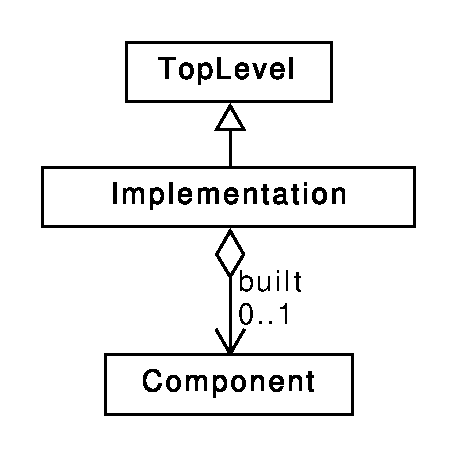
\includegraphics[scale=0.65]{uml/implementation}
\caption[]{Diagram of the \sbol{Implementation} class and its associated properties.}
\label{uml:implementation}
\end{center}
\end{figure}

\subparagraph{The \sbolheading{built} property}\label{sec:built}
The \sbol{built} property is OPTIONAL and MAY contain a URI that MUST refer to a \sbol{Component}. This \sbol{Component} is intended to describe the actual physical structure and/or functional behavior of the \sbol{Implementation}. When the built property refers to a \sbol{Component} that is also linked to the \sbol{Implementation} via PROV-O properties such as \prov{wasDerivedFrom} (see \ref{sec:provenance}), it can be inferred that the actual structure and/or function of the \sbol{Implementation} matches its original design. When the \sbol{built} property refers to a different \sbol{Component}, it can be inferred that the \sbol{Implementation} has deviated from the original design. For example, the latter could be used to document when the DNA sequencing results for an assembled construct do not match the original target sequence.


